%  A simple AAU report template.
%  2015-05-08 v. 1.2.0
%  Copyright 2010-2015 by Jesper Kjær Nielsen <jkn@es.aau.dk>
%  Modified 2025 by Viktor Kirk Almann Hansen <vhanse23@student.aau.dk>
%
%  This is free software: you can redistribute it and/or modify
%  it under the terms of the GNU General Public License as published by
%  the Free Software Foundation, either version 3 of the License, or
%  (at your option) any later version.
%
%  This is distributed in the hope that it will be useful,
%  but WITHOUT ANY WARRANTY; without even the implied warranty of
%  MERCHANTABILITY or FITNESS FOR A PARTICULAR PURPOSE.  See the
%  GNU General Public License for more details.
%
%  You can find the GNU General Public License at <http://www.gnu.org/licenses/>.
%
%  A simple AAU report template.
%  2015-05-08 v. 1.2.0
%  Copyright 2010-2015 by Jesper Kjær Nielsen <jkn@es.aau.dk>
%  Modified 2025 by Viktor Kirk Almann Hansen <vhanse23@student.aau.dk>
%
%  This is free software: you can redistribute it and/or modify
%  it under the terms of the GNU General Public License as published by
%  the Free Software Foundation, either version 3 of the License, or
%  (at your option) any later version.
%
%  This is distributed in the hope that it will be useful,
%  but WITHOUT ANY WARRANTY; without even the implied warranty of
%  MERCHANTABILITY or FITNESS FOR A PARTICULAR PURPOSE.  See the
%  GNU General Public License for more details.
%
%  You can find the GNU General Public License at <http://www.gnu.org/licenses/>.
%
\documentclass[11pt,a4paper,openright]{report}
%%%%%%%%%%%%%%%%%%%%%%%%%%%%%%%%%%%%%%%%%%%%%%%%
% Language, Encoding and Fonts
% http://en.wikibooks.org/wiki/LaTeX/Internationalization
%%%%%%%%%%%%%%%%%%%%%%%%%%%%%%%%%%%%%%%%%%%%%%%%
% Select encoding of your inputs. Depends on
% your operating system and its default input
% encoding. Typically, you should use
%   Linux  : utf8 (most modern Linux distributions)
%            latin1 
%   Windows: ansinew
%            latin1 (works in most cases)
%   Mac    : applemac
% Notice that you can manually change the input
% encoding of your files by selecting "save as"
% an select the desired input encoding. 

% Make latex understand and use the typographic
% rules of the language used in the document.
\usepackage[australian]{babel}
% Use the palatino font
\usepackage[sc]{mathpazo}
\linespread{1.2}         % Palatino needs more leading (space between lines)
% Choose the font encoding
\usepackage[T1]{fontenc}
\usepackage{multirow}
\usepackage{multicol}
%%%%%%%%%%%%%%%%%%%%%%%%%%%%%%%%%%%%%%%%%%%%%%%%
% Graphics and Tables
% http://en.wikibooks.org/wiki/LaTeX/Importing_Graphics
% http://en.wikibooks.org/wiki/LaTeX/Tables
% http://en.wikibooks.org/wiki/LaTeX/Colors
%%%%%%%%%%%%%%%%%%%%%%%%%%%%%%%%%%%%%%%%%%%%%%%%
% load a colour package
\usepackage{xcolor}
\definecolor{aaublue}{RGB}{33,26,82}% dark blue
% The standard graphics inclusion package
\usepackage{graphicx}
% Set up how figure and table captions are displayed
\usepackage{caption}
\captionsetup{%
  font=footnotesize,% set font size to footnotesize
  labelfont=bf % bold label (e.g., Figure 3.2) font
}
% Make the standard latex tables look so much better
\usepackage{array,booktabs}
% Enable the use of frames around, e.g., theorems
% The framed package is used in the example environment
\usepackage{framed}

\usepackage{wrapfig}

\usepackage{tabularx}

\usepackage{listings}

\definecolor{codegreen}{rgb}{0,0.6,0}
\definecolor{codegray}{rgb}{0.5,0.5,0.5}
\definecolor{codepurple}{rgb}{0.58,0,0.82}
\definecolor{backcolour}{rgb}{0.95,0.95,0.92}

\lstdefinestyle{mystyle}{
  backgroundcolor=\color{backcolour}, commentstyle=\color{codegreen},
  keywordstyle=\color{magenta},
  numberstyle=\tiny\color{codegray},
  stringstyle=\color{codepurple},
  basicstyle=\ttfamily\footnotesize,
  breakatwhitespace=false,         
  breaklines=true,                 
  captionpos=b,                    
  keepspaces=true,                 
  numbers=left,                    
  numbersep=5pt,                  
  showspaces=false,                
  showstringspaces=false,
  showtabs=false,                  
  tabsize=2
}
\lstdefinestyle{mystyle2}{
  commentstyle=\color{gray},          % Comments in gray
  keywordstyle=\color{blue},         % Keywords in blue
  stringstyle=\color{teal},          % Strings in teal
  basicstyle=\ttfamily\footnotesize, % Monospaced font, smaller size
  frame=lines,                       % Simple lines above and below
  framesep=2mm,                      % Small space between frame and text
  rulecolor=\color{black},           % Black frame lines
  breaklines=true,                   % Enable line breaking
  captionpos=b,                      % Captions below the code
  keepspaces=true,                   % Preserve spaces in code
  numbers=left,                      % Line numbers on the left
  numbersep=10pt,                    % Space between line numbers and code
  tabsize=2,                         % Tab width
  showspaces=false,                  % Don't show spaces
  showstringspaces=false,            % Don't show spaces in strings
  showtabs=false,                    % Don't show tabs
}


\lstset{style=mystyle}

\makeatletter
\let\orig@lstnumber=\thelstnumber

\newcommand\lstsetnumber[1]{\gdef\thelstnumber{#1}}
\newcommand\lstresetnumber{\global\let\thelstnumber=\orig@lstnumber}
\makeatother

\usepackage{xcolor}
\newcommand{\myRed}[1]{\textcolor{red}{#1}}
\newcommand{\vc}[1]{\textcolor{orange}{#1}}

\usepackage[acronym]{glossaries}
%%%%%%%%%%%%%%%%%%%%%%%%%%%%%%%%%%%%%%%%%%%%%%%%
% Mathematics
% http://en.wikibooks.org/wiki/LaTeX/Mathematics
%%%%%%%%%%%%%%%%%%%%%%%%%%%%%%%%%%%%%%%%%%%%%%%%
% Defines new environments such as equation,
% align and split 
\usepackage{amsmath}
% Adds new math symbols
\usepackage{amssymb}
% Use theorems in your document
% The ntheorem package is also used for the example environment
% When using thmmarks, amsmath must be an option as well. Otherwise \eqref doesn't work anymore.
\usepackage[framed,amsmath,thmmarks]{ntheorem}
%%%%%%%%%%%%%%%%%%%%%%%%%%%%%%%%%%%%%%%%%%%%%%%%
% Page Layout
% http://en.wikibooks.org/wiki/LaTeX/Page_Layout
%%%%%%%%%%%%%%%%%%%%%%%%%%%%%%%%%%%%%%%%%%%%%%%%
\usepackage{eso-pic}
% Change margins, papersize, etc of the document
\usepackage[
  inner=28mm,% left margin on an odd page
  outer=28mm,% right margin on an odd page, default: 41
  ]{geometry}
% Modify how \chapter, \section, etc. look
% The titlesec package is very configureable

\usepackage{titlesec}
\titleformat{\chapter}[hang]
{\vspace{-7\baselineskip}\normalfont\huge\bfseries}
{\fontsize{26}{30}\selectfont\thechapter.}
{20pt}
{\Huge}
\titlespacing*{\chapter}{0pt}{45pt}{15pt}



\titleformat*{\section}{\normalfont\Large\bfseries}
\titleformat*{\subsection}{\normalfont\large\bfseries}
\titleformat*{\subsubsection}{\normalfont\normalsize\bfseries}
%\titleformat*{\paragraph}{\normalfont\normalsize\bfseries}
%\titleformat*{\subparagraph}{\normalfont\normalsize\bfseries}

% Clear empty pages between chapters


% Change the headers and footers
\usepackage{fancyhdr}
\pagestyle{fancy}
\fancyhf{} %delete everything
\renewcommand{\headrulewidth}{0pt} %remove the horizontal line in the header
\fancyhead[R]{\small\nouppercase\leftmark} %even page - chapter title
\fancyhead[L]{\small\nouppercase\rightmark} %uneven page - section title
\fancyfoot[C]{\thepage} % Page number centered in footer
% Do not stretch the content of a page. Instead,
% insert white space at the bottom of the page
\raggedbottom
% Enable arithmetics with length. Useful when
% typesetting the layout.
\usepackage{calc}
\usepackage{tikz}

%%%%%%%%%%%%%%%%%%%%%%%%%%%%%%%%%%%%%%%%%%%%%%%%
% Bibliography
% http://en.wikibooks.org/wiki/LaTeX/Bibliography_Management
%%%%%%%%%%%%%%%%%%%%%%%%%%%%%%%%%%%%%%%%%%%%%%%%
\usepackage[
  backend=biber,
  bibencoding=utf8,
  sorting=none,
  style=numeric,
  language=australian
  ]{biblatex}
\addbibresource{bib/references.bib}

%%%%%%%%%%%%%%%%%%%%%%%%%%%%%%%%%%%%%%%%%%%%%%%%
% Misc
%%%%%%%%%%%%%%%%%%%%%%%%%%%%%%%%%%%%%%%%%%%%%%%%
% Space instead of indent
\usepackage[parfill]{parskip}

\usepackage[skins,minted]{tcolorbox}



\definecolor{mintedbackground}{rgb}{0.95,0.95,0.95}
\definecolor{mintedframe}{rgb}{0.70,0.85,0.95}

% This is the bash profile used throughout the document.
% I've also got one for Python and console text (regular commands)
\setminted[bash]{
    bgcolor=white,
    fontfamily=tt,
    linenos=true,
    numberblanklines=true,
    numbersep=12pt,
    numbersep=5pt,
    gobble=0,
    frame=leftline,
    framesep=2mm,
    funcnamehighlighting=true,
    tabsize=4,
    obeytabs=false,
    mathescape=false
    samepage=false,
    showspaces=false,
    showtabs =false,
    texcl=false,
    baselinestretch=1.2,
    breaklines=true,
}

\newtcblisting{myminted}[2][]{enhanced, listing engine=minted, 
listing only,#1, title=#2, minted language=bash, 
coltitle=mintedbackground!30!black, 
fonttitle=\ttfamily\footnotesize,
sharp corners, top=0mm, bottom=0mm,
title code={\path[draw=mintedframe,dashed, fill=mintedbackground](title.south west)--(title.south east);},
frame code={\path[draw=mintedframe, fill=mintedbackground](frame.south west) rectangle (frame.north east);}
}





\setcounter{tocdepth}{2}
% Add bibliography and index to the table of
% contents
\usepackage[nottoc]{tocbibind}
% Add the command \pageref{LastPage} which refers to the
% page number of the last page
\usepackage{lastpage}
% Add todo notes in the margin of the document
\usepackage[
%  disable, %turn off todonotes
  colorinlistoftodos, %enable a coloured square in the list of todos
  textwidth=\marginparwidth, %set the width of the todonotes
  textsize=scriptsize, %size of the text in the todonotes
  ]{todonotes}

\usepackage{tabto} %Allows tab function.

\usepackage{graphicx,subcaption,lipsum}

%%%%%%%%%%%%%%%%%%%%%%%%%%%%%%%%%%%%%%%%%%%%%%%%
% Hyperlinks
% http://en.wikibooks.org/wiki/LaTeX/Hyperlinks
%%%%%%%%%%%%%%%%%%%%%%%%%%%%%%%%%%%%%%%%%%%%%%%%
% Enable hyperlinks and insert info into the pdf
% file. Hypperref should be loaded as one of the 
% last packages
\usepackage[pdfborder={0 0 0}]{hyperref}
\hypersetup{%
	plainpages=false,%
	pdfauthor={Author(s)},%
	pdftitle={Title},%
	pdfsubject={Subject},%
	bookmarksnumbered=true,%
	colorlinks=false,%
	citecolor=black,%
	filecolor=black,%
	linkcolor=black,% you should probably change this to black before printing
	urlcolor=black,%
	pdfstartview=FitH%
}
\makeglossaries


\makeatletter
\newcommand*{\centerfloat}{%
  \parindent \z@
  \leftskip \z@ \@plus 1fil \@minus \textwidth
  \rightskip\leftskip
  \parfillskip \z@skip}
\makeatother


\setcounter{tocdepth}{1} %shows the subsections in the ToC

\usepackage{csquotes}
\usepackage{datetime} % Til korrekt visning af tid og dato
\usepackage{tablefootnote} % fordi latex er øv nogle gange
\usepackage{threeparttable} % same
\usepackage{makecell} % Add this line in your preamble
\usepackage{enumitem}
\newenvironment{bfenumerate}[1][]
 {\begin{enumerate}[before=\bfseries,#1]}
 {\end{enumerate}}
\interfootnotelinepenalty=10000 % fix funky footnotes 

\captionsetup{justification=centering}
\usepackage{fancyvrb}

\usepackage{enumitem}
\setlist[itemize]{topsep=0pt, parsep=0pt, itemsep=4pt}
\setlist[enumerate]{topsep=0pt, parsep=0pt, itemsep=5pt}



\usepackage{pgfkeys,pgfcalendar}
\newcount\pgfdatecount
\newcommand{\tomorrow}{%
\pgfcalendardatetojulian{\year-\month-\day+1}{\pgfdatecount}
\pgfcalendarjuliantodate{\the\pgfdatecount}{\myyear}{\mymonth}{\myday}
\pgfcalendarmonthname{\mymonth}\space\myday,\space\myyear%
}


\usepackage{pdfpages}
\usepackage[table]{xcolor} % For shading rows
% Packages for writing
\usepackage{enumitem}

\newenvironment{conditions}
  {\par\vspace{\abovedisplayskip}\noindent\begin{tabular}{>{$}l<{$} @{${}={}$} l}}
  {\end{tabular}\par\vspace{\belowdisplayskip}}% package inclusion and set up of the document
% see, e.g., http://en.wikibooks.org/wiki/LaTeX/Formatting#Hyphenation
% for more information on word hyphenation
\hyphenation{ex-am-ple hy-phen-a-tion short}
\hyphenation{long la-tex}
\hyphenation{trans-ceivers}
\hyphenation{auto-nomous}
% 
%  A simple AAU report template.
%  2015-05-08 v. 1.2.0
%  Copyright 2010-2015 by Jesper Kjær Nielsen <jkn@es.aau.dk>
%  Modified 2025 by Viktor Kirk Almann Hansen <vhanse23@student.aau.dk>
%
%  This is free software: you can redistribute it and/or modify
%  it under the terms of the GNU General Public License as published by
%  the Free Software Foundation, either version 3 of the License, or
%  (at your option) any later version.
%
%  This is distributed in the hope that it will be useful,
%  but WITHOUT ANY WARRANTY; without even the implied warranty of
%  MERCHANTABILITY or FITNESS FOR A PARTICULAR PURPOSE.  See the
%  GNU General Public License for more details.
%
%  You can find the GNU General Public License at <http://www.gnu.org/licenses/>.
%
%
%
% see, e.g., http://en.wikibooks.org/wiki/LaTeX/Customizing_LaTeX#New_commands
% for more information on how to create macros

%%%%%%%%%%%%%%%%%%%%%%%%%%%%%%%%%%%%%%%%%%%%%%%%
% Macros for the titlepage
%%%%%%%%%%%%%%%%%%%%%%%%%%%%%%%%%%%%%%%%%%%%%%%%
%Creates the aau titlepage
\newcommand{\aautitlepage}[3]{%
  {
    %set up various length
    \ifx\titlepageleftcolumnwidth\undefined
      \newlength{\titlepageleftcolumnwidth}
      \newlength{\titlepagerightcolumnwidth}
    \fi
    \setlength{\titlepageleftcolumnwidth}{0.5\textwidth-\tabcolsep}
    \setlength{\titlepagerightcolumnwidth}{\textwidth-2\tabcolsep-\titlepageleftcolumnwidth}
    \vspace*{-3.5cm}
    %create title page
    \enlargethispage{\baselineskip}
    \noindent%
    \begin{tabular}{@{}ll@{}}
      \parbox{\titlepageleftcolumnwidth}{
        \iflanguage{danish}{%
          
\includegraphics[width=\titlepageleftcolumnwidth]{figures/AAUgraphics/aau_logo_da}
        }{%
          
\includegraphics[width=\titlepageleftcolumnwidth]{figures/AAUgraphics/aau_logo_en}
        }
      } &
      \parbox{\titlepagerightcolumnwidth}{\raggedleft\sf\small
        #2
      }\bigskip\\
       #1 &
      \parbox[t]{\titlepagerightcolumnwidth}{%
      \textbf{Abstract:}\bigskip\par
        \fbox{\parbox{\titlepagerightcolumnwidth-1\fboxsep-2\fboxrule}{%
          #3
        }}
      }\\
    \end{tabular}
    \vfill
    \iflanguage{danish}{%
      \noindent{\footnotesize\emph{Rapportens indhold er frit tilgængeligt, men offentliggørelse (med kildeangivelse) må kun ske efter aftale med forfatterne.}}
    }{%
        
      \noindent{\footnotesize\emph{The content of this report is freely available, but publication (with reference) may only be pursued due to agreement with the authors.}}
    }
  }
}

%Create english project info
\newcommand{\englishprojectinfo}[8]{%
  \parbox[t]{\titlepageleftcolumnwidth}{
    \textbf{Title:}\\ #1\bigskip\par
    \textbf{Theme:}\\ #2\bigskip\par
    \textbf{Project Period:}\\ #3\bigskip\par
    \textbf{Project Group:}\\ #4\bigskip\par
    \textbf{Participant(s):}\\ #5\bigskip\par
    \textbf{Supervisor(s):}\\ #6\bigskip\par
    \textbf{Page Numbers:} \pageref{LastPage}\bigskip\par
    \textbf{Date of Completion:}\\ #7
  }
}

%Create danish project info
\newcommand{\danishprojectinfo}[8]{%
  \parbox[t]{\titlepageleftcolumnwidth}{
    \textbf{Titel:}\\ #1\bigskip\par
    \textbf{Tema:}\\ #2\bigskip\par
    \textbf{Projektperiode:}\\ #3\bigskip\par
    \textbf{Projektgruppe:}\\ #4\bigskip\par
    \textbf{Deltager(e):}\\ #5\bigskip\par
    \textbf{Vejleder(e):}\\ #6\bigskip\par
    \textbf{Sidetal:} \pageref{LastPage}\bigskip\par
    \textbf{Afleveringsdato:}\\ #7
  }
}

%%%%%%%%%%%%%%%%%%%%%%%%%%%%%%%%%%%%%%%%%%%%%%%%
% An example environment
%%%%%%%%%%%%%%%%%%%%%%%%%%%%%%%%%%%%%%%%%%%%%%%%
% my new macros 
\setlength {\marginparwidth }{2cm}
\begin{document}
%frontmatter
\pagestyle{empty} %disable headers and footers
\pagenumbering{roman} %use roman page numbering in the frontmatter


\pdfbookmark[0]{Front page}{label:frontpage}%
\begin{titlepage}
\vspace*{\fill}
    \AddToShipoutPictureBG*{%
        \AtPageLowerLeft{%
            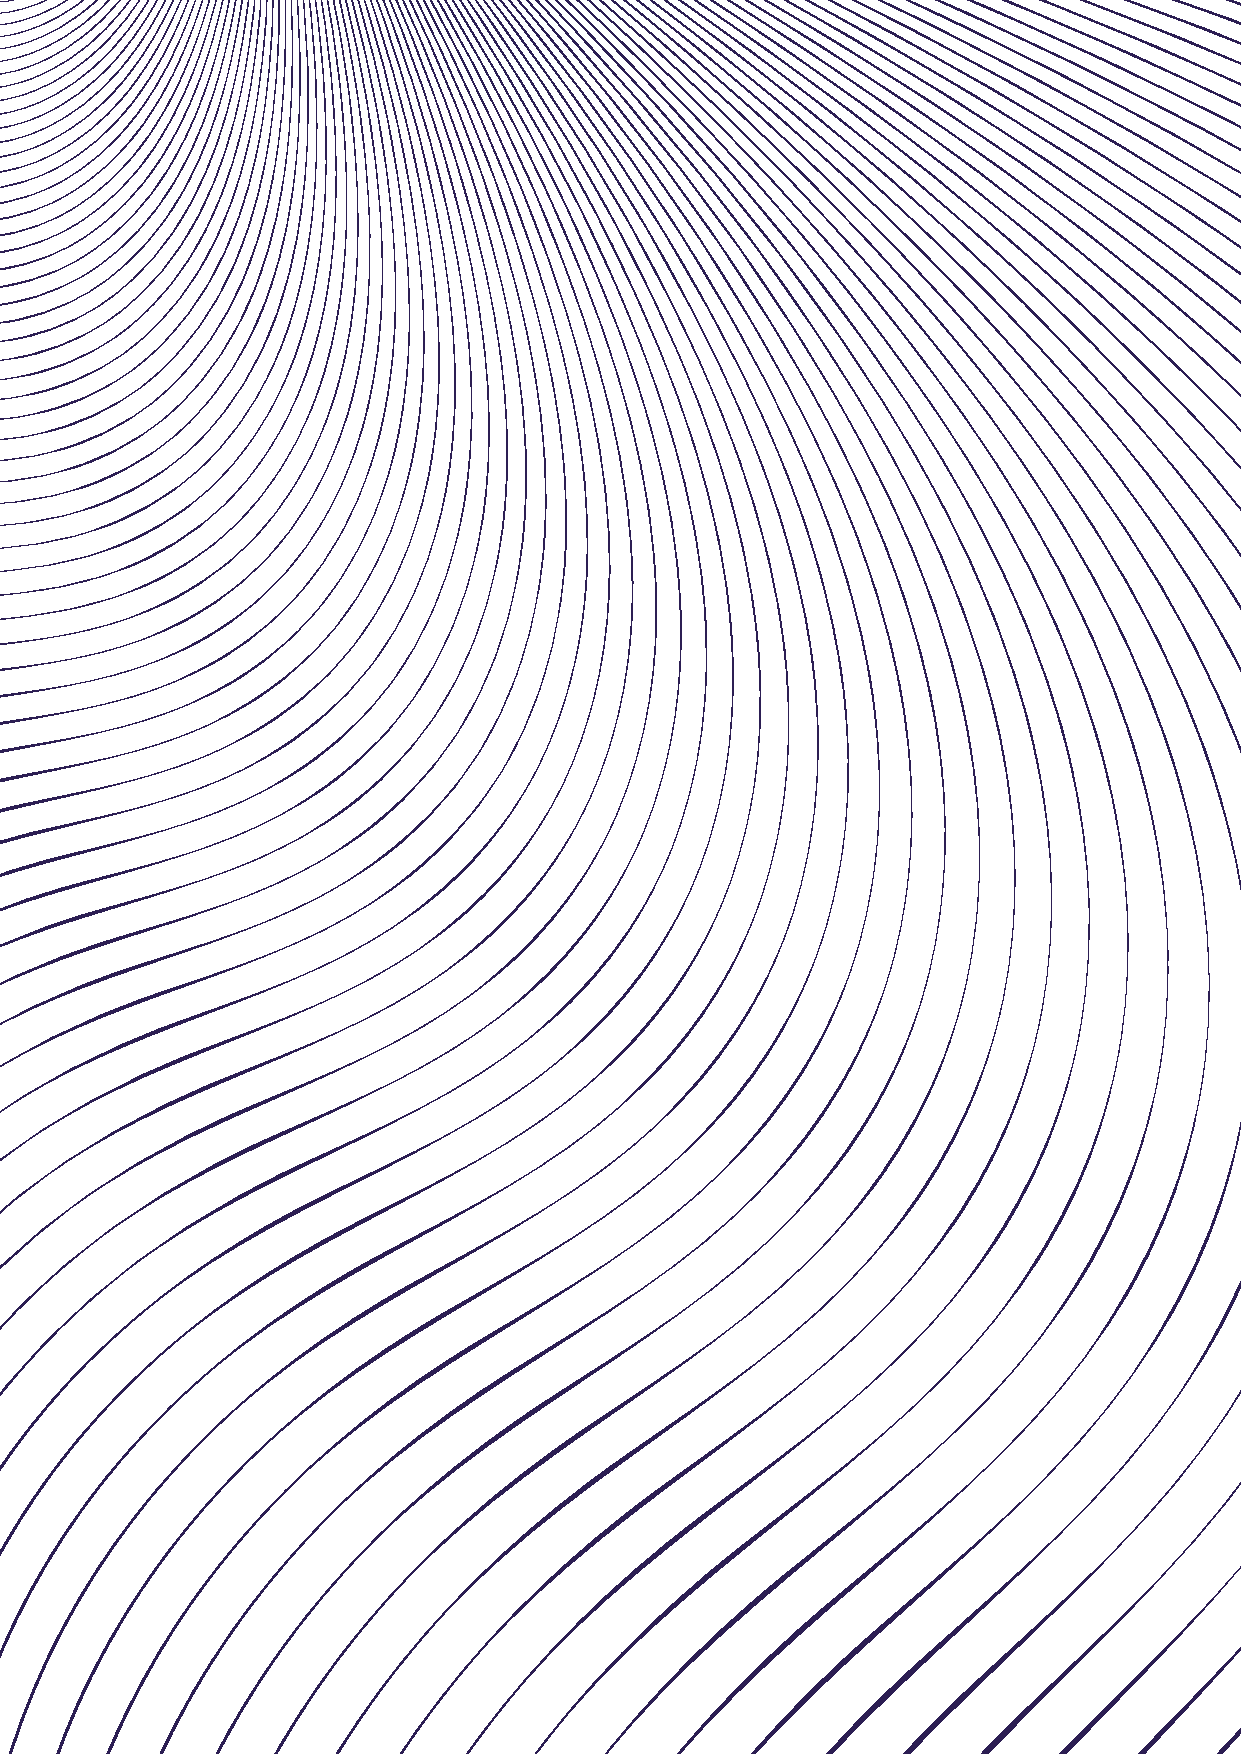
\includegraphics[width=\paperwidth,height=\paperheight]{figures/AAUgraphics/aau_waves}%
        }%
    }
  \addtolength{\hoffset}{0.5\evensidemargin-0.5\oddsidemargin} %set equal margins on the frontpage - remove this line if you want default margins
  \noindent%
  {\color{white}\fboxsep5pt\colorbox{aaublue}{\begin{tabular}{@{}p{\textwidth}@{}}
    \begin{center}
    \Huge{\textbf{
      Title % insert your title here
    }}
    \end{center}
    \begin{center}
      \Large{
       Sub-title   % insert your subtitle here
      }
    \end{center}
    \vspace{0.5cm}
   \begin{center}
    \vspace{0.5cm}
    {\large
      Computer Engineering \\
      Group ?? \\
      \today 
      % insert name of study, group number, year-month
    }
   \end{center}
   \vspace{0.5cm}
%% Comment this section in if you are doing Bachelor or Master Project   
   \begin{center}
    {\Large
      P?? Project
      %
    }
   \end{center}
\end{tabular}}}
  \vfill
  \begin{center}
    
\includegraphics[width=0.2\paperwidth]{figures/AAUgraphics/aau_logo_circle_en}% comment this line in for English version
    %
\includegraphics[width=0.2\paperwidth]{AAUgraphics/aau_logo_circle_da} %comment this line in for Danish version
  \end{center}
\end{titlepage}
\clearpage

\pdfbookmark[0]{English title page}{label:titlepage_en}
\aautitlepage{%
  \englishprojectinfo{
    Title %title
  }{%
    Scientific Theme %theme
  }{%
    Spring/Fall Semester 202?? %project period
  }{%
    Group ?? % project group
  }{%
    %list of group members
    Name1 (study number)         \\
    Name2 (study number)     \\
    ...
  }{%
    %list of supervisors
    Supervisor1  \\
    Supervisor2
  }{%
    \today % date of completion
  }%
}{%department and address
  \textbf{Electronics and IT}\\
  Aalborg University\\
  \href{https://www.aau.dk}{https://www.aau.dk}
}{  
    ??
}

\glsresetall 

\newglossaryentry{latex}{
    name=LaTeX,
    description={A document preparation system for high-quality typesetting}
}

\newacronym{usb}{USB}{Universal Serial Bus}


%%% Actually shows the glossary
\printglossary[type=\acronymtype]
\printglossary

\pdfbookmark[0]{Contents}{label:contents}
\pagestyle{fancy} %enable headers and footers again
\tableofcontents
\addtocontents{toc}{\protect\enlargethispage{\baselineskip}}
\chapter*{Preface\markboth{Preface}{Preface}}\label{ch:preface}
\addcontentsline{toc}{chapter}{Preface}
The code developed and used in this project can be found on \href{link_to_git}{GitHub}\footnote{\url{link_to_git}}.

% We would like to thank redwine for the great support throughout the project and life in general. This projct have been completed without the sublime support of redwine. 

\vspace{\baselineskip}\hfill Aalborg University, \today
\vspace{2cm}

\begin{minipage}[b]{0.45\textwidth}
 \centering
 \raisebox{-0.5\height}
 {
\includegraphics[width=1\textwidth]{figures/signatures/empty_signature.png}}
 \rule{\textwidth}{0.5pt}\\
  Name1\\
  {\footnotesize student mail}
\end{minipage}
\hfill
\begin{minipage}[b]{0.45\textwidth}
 \centering 
 \raisebox{-0.5\height}
 {
\includegraphics[width=1\textwidth]{figures/signatures/empty_signature.png}}
 \rule{\textwidth}{0.5pt}\\
  Name2\\
  {\footnotesize student mail}
\end{minipage}

\vspace{1,75cm}

\begin{minipage}[b]{0.45\textwidth}
 \centering
 \raisebox{-0.5\height}
 {
\includegraphics[width=1\textwidth]{figures/signatures/empty_signature.png}}
 \rule{\textwidth}{0.5pt}\\
  Name3\\
  {\footnotesize student mail}
\end{minipage}
\hfill
\begin{minipage}[b]{0.45\textwidth}
 \centering
 \raisebox{-0.5\height}
 {
\includegraphics[width=1\textwidth]{figures/signatures/empty_signature.png}}
 \rule{\textwidth}{0.5pt}\\
  Name4\\
  {\footnotesize student mail}
\end{minipage}


\vspace{1\baselineskip}



\thispagestyle{empty}
{\small
\strut\vfill % push the content to the bottom of the page
\noindent Copyright \copyright{} Aalborg University \THEYEAR\par
\vspace{0.2cm}
\noindent In this report, generative AI has been used as a consulting tool, aiding with code suggestions and refinement, as well as a general consulting partner.


}

\clearpage
%\cleardoublepage



% mainmatter
\pagenumbering{arabic} %use arabic page numbering in the mainmatter
\chapter{Introduction} \label{ch:introduction}

Welcome! This is the template I use when writing reports in \LaTeX.  
Below you can find some key elements that are useful when writing.  

All the text you write should go into the \texttt{.tex} files you see on the left.  
In \texttt{master.tex} you can include new \texttt{.tex} files to be compiled into the PDF (take a look in that file to see how it works).  
In \texttt{preamble.tex} you can add new packages for extra features and commands.  

To see changes in the PDF, recompile by pressing the compile button or using \texttt{Ctrl+S}.  
You can use the arrows between the editor and PDF to navigate to specific pages, and you can double-click inside the PDF to jump to where that part was written in the code.  

---

\section*{Comments}
To comment something out (so it won’t show in the PDF), use:

% This won't be in the PDF

You can also use the \texttt{comment} environment:

\begin{comment}
    This also won't be in the PDF
\end{comment}

\section*{Line breaks}
To go to the next line without starting a new paragraph, use:

Line one \\
Line two

A double line break creates a new paragraph.

\section*{Symbols}
To write special characters, use a backslash in front of them:
\% \& \# \_
For a backslash itself, use: \textbackslash.

\newpage
\section*{Lists}
You can create bullet lists with \texttt{itemize}:

\begin{itemize}
    \item First item
    \item Second item
\end{itemize}
Or numbered lists with \texttt{enumerate}:

\begin{enumerate}
    \item First item
    \item Second item
\end{enumerate}
You can also customize the numbering style:

\begin{enumerate}[label=\alph*]
    \item Item a
    \item Item b
\end{enumerate}


\chapter*{Chapters and sections} \label{ch:placeholder}
You can structure your document like this:

\section*{New section} \label{sec:placeholder}
Putting a \* after the section or chapter will not give a number and not add it to the table of contents (Which updates automatically).

\subsection*{New subsection} \label{sec:sub_placeholder}

\subsubsection{New subsubsection} \label{sec:subsub_placeholder}
Note: subsubsection does not get a number by default.

To force a page break use:
\newpage



\section*{Tables}
Here is an example of a table:

\begin{table}[H]
    \centering
    \begin{tabular}{cc}
        \toprule
        \textbf{Column 1} & \textbf{Column 2} \\
        \midrule
        1  & a \\
        2  & b \\
        3  & c \\
        4  & d \\
        5  & e \\
        6  & f \\
        \bottomrule
    \end{tabular}
    \caption{Caption for the table...}
    \label{tab:placeholder}
\end{table}
There is so many ways to do it, you can look up online latex table editors/generators to customize them.

\section*{Figures}

To make a figure you can just copy a image with ctrl-c and paste it in with ctrl-v and the following will appear, you can also manually add them to the folder "figures/images" and then write the stuff below where you change the image name.

\begin{figure}[H]
    \centering
    
\includegraphics[width=0.75\linewidth]{figures/images/pikachu.jpg}
    \caption{Caption for the figure}
    \label{fig:placeholder}
\end{figure}

\section*{Labels and references}
It’s important to add labels to chapters, sections, figures, and tables so you can reference them later.

Examples:

See Figure \ref{fig:placeholder},  
as shown in Table \ref{tab:placeholder},  
or as explained in Chapter \ref{ch:conclusion}.
In the PDF, you can click the reference numbers to jump to the corresponding place. Always make a reference to a figure, table, equation or what else you add.



\section*{Math equations}

You can write inline math like this: $E = mc^2$.  
Or display math like this:
\[
    \int_0^1 x^2 \, dx = \frac{1}{3}
\]
Another way is to use the equation environment (you can add labels to this and reference to it):
\begin{equation}
    a^2 + b^2 = c^2
\end{equation}

Or:
$$ a^2 + b^2 = c^2 $$



\section*{Code snippets}

To insert code, you can use the verbatim environment:
\begin{verbatim}
print("Hello, world!")
for i in range(5):
    print(i)
\end{verbatim}

Or with listings:
\begin{lstlisting}[language=Python, caption=Example Python code]
def hello():
    print("Hello, LaTeX!")
\end{lstlisting}

There is many other ways to do it as well feel free to google.


\section*{Glossary}

The glossary entries are defined in the file \texttt{glossary.tex}.  
You can reference them in the text with the command, \gls{latex}.  
The corresponding explanation will appear in the glossary before the table of contents.  

Acronyms can also be added. For instance, the acronym USB is defined in the glossary: the first use of \gls{usb} will produce the full form, while subsequent uses will display the short form. Using this convention makes the report more consistent and easier to read.


\section*{Citations}

To cite references, create a .bib file and add a entry.

Then cite it in your text with \cite{lamport1994}. 


A way smarter way to handle references/citations is to use the program Zotero. This is a fantastic tool that you have to install on you pc and add a browser extension for. Google this to learn it or ask me.


\section*{Project Folder Structure}

The project is organized into the following folders and files:

\begin{itemize}
    \item \textbf{.tex files}: Used for writing the main report content.
    \item \textbf{appendix/}: Contains \texttt{.tex} files and any PDFs that should be included in the appendix.
    \item \textbf{bib/}: Contains the bibliography files for references (I put my Zotero imported references.bib here).
    \item \textbf{figures/AAUgraphics/}: Contains AAU logos and templates.
    \item \textbf{figures/draw.io\_files/}: I use it to store my groups original diagram source files (created in draw.io), in case modifications are needed later.
    \item \textbf{figures/images/}: Contains figures, images, diagrams etc.
    \item \textbf{figures/signatures/}: Contains the groups signatures for the Preface.
    \item \textbf{sections/}: Holds the \texttt{.tex} files for each report section. A common convention is to name them after the corresponding chapter number.
    \item \textbf{setup/}: Controls how the PDF is compiled and which packages are loaded.
    \item \textbf{master.tex}: The main file that assembles the entire report into a single PDF. 
    It is important to set \texttt{master.tex} as the main document in your LaTeX editor to ensure the PDF compiles correctly.
\end{itemize}


\chapter{Problem Analysis} \label{ch:problem}
\chapter{Concept Specification} \label{ch:concept}


\chapter{System Design} \label{ch:system_design}


\chapter{System Implementation} \label{ch:system_implementation}


\chapter{System Validation}\label{ch:test}


\chapter{Discussion} \label{ch:discussion}


\chapter{Conclusion} \label{ch:conclusion}



\printbibliography[heading=bibintoc, title=Bibliography]
\label{bib:mybiblio}

\appendix
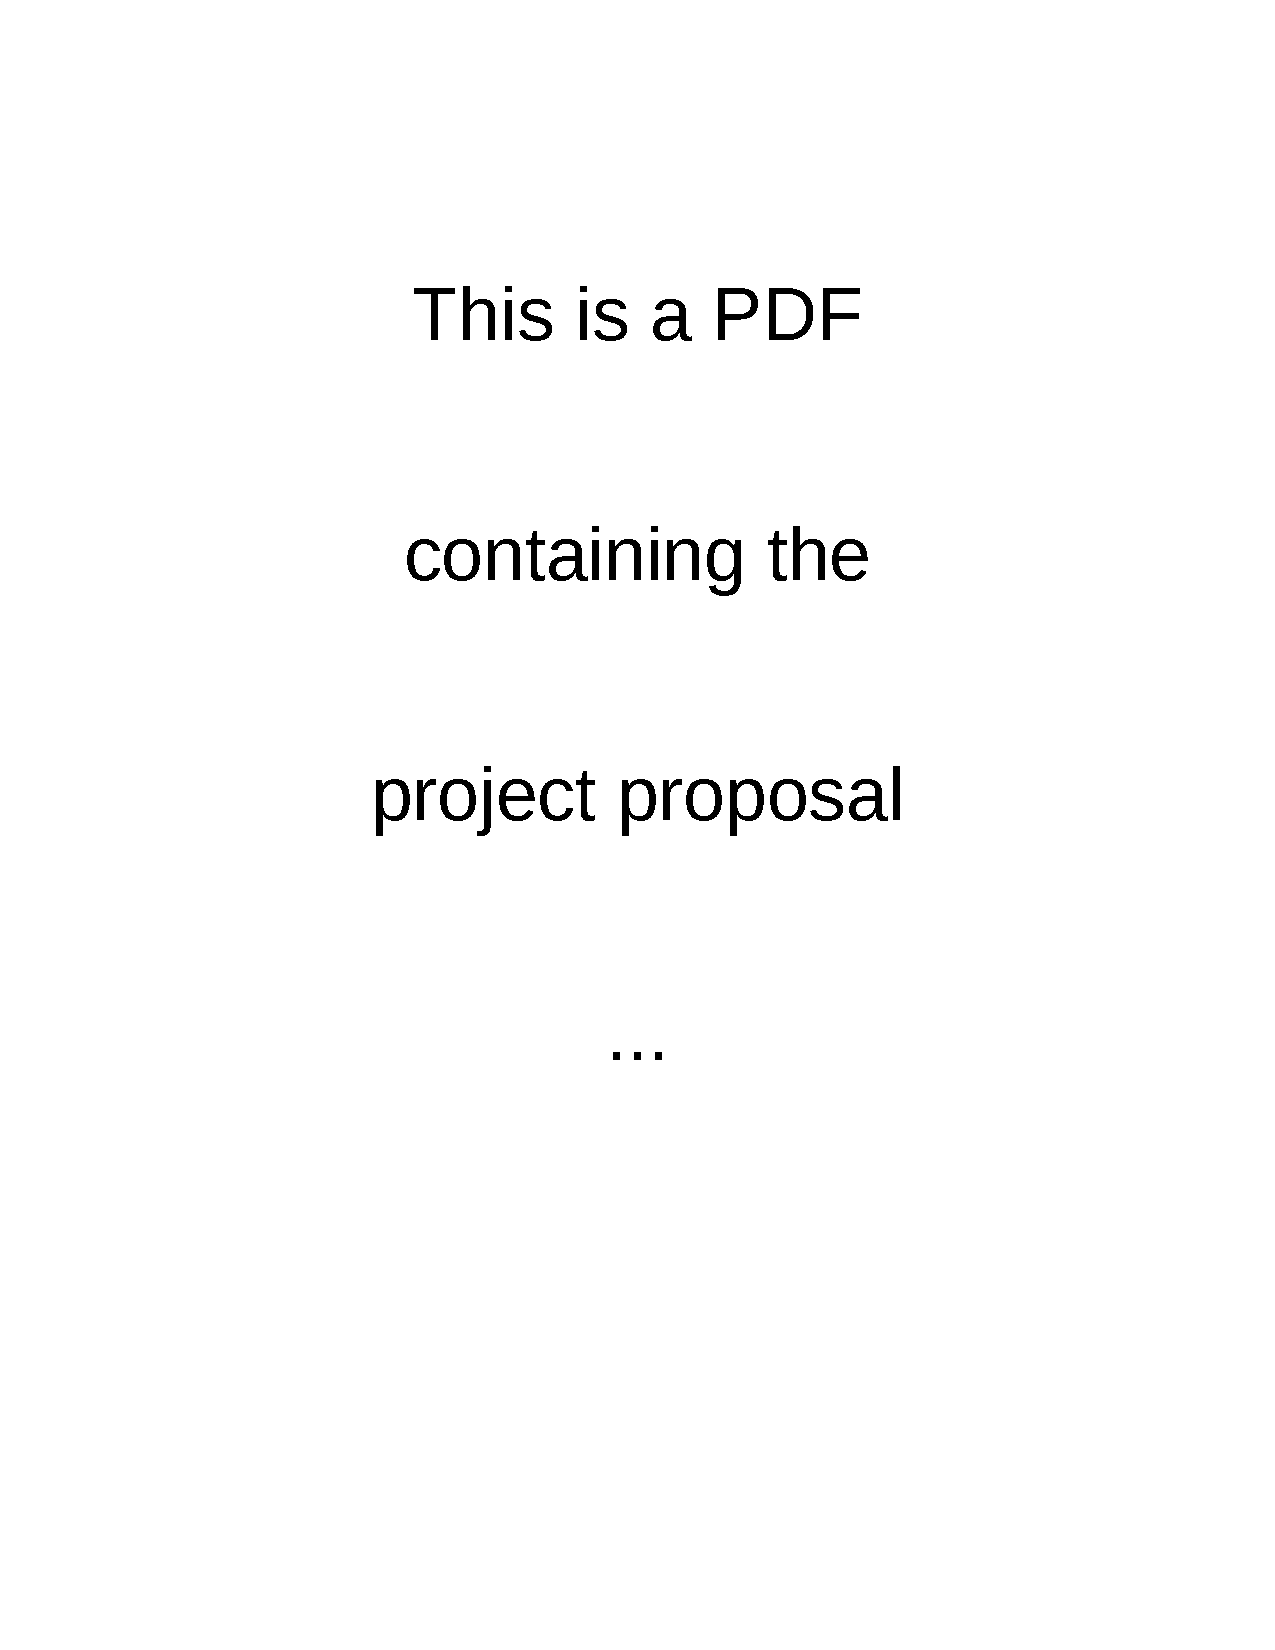
\includepdf[pages=-, pagecommand={\chapter{Project Proposal\label{app:proposal}}}]{appendix/project_proposal.pdf}
\chapter{Other stuff in appendix}

% You can add whatever you want here...
\chapter{Meeting Notes}

% I don't put this in the appendix when submitting the rapport, however it helps to have notes from all meetings, when making the project.

% To remove this from the compilled PDF go into master.tex and comment out the "\chapter{Meeting Notes}

% I don't put this in the appendix when submitting the rapport, however it helps to have notes from all meetings, when making the project.

% To remove this from the compilled PDF go into master.tex and comment out the "\chapter{Meeting Notes}

% I don't put this in the appendix when submitting the rapport, however it helps to have notes from all meetings, when making the project.

% To remove this from the compilled PDF go into master.tex and comment out the "\input{appendix/meeting_notes}"


\section{
    Introductory meeting DATE (Participants)
}

\begin{itemize}
    \item ...
\end{itemize}


\clearpage\newpage


\section{
    Meeting DATE (Participants)
}

\begin{itemize}
    \item ...
\end{itemize}


\clearpage\newpage
"


\section{
    Introductory meeting DATE (Participants)
}

\begin{itemize}
    \item ...
\end{itemize}


\clearpage\newpage


\section{
    Meeting DATE (Participants)
}

\begin{itemize}
    \item ...
\end{itemize}


\clearpage\newpage
"


\section{
    Introductory meeting DATE (Participants)
}

\begin{itemize}
    \item ...
\end{itemize}


\clearpage\newpage


\section{
    Meeting DATE (Participants)
}

\begin{itemize}
    \item ...
\end{itemize}


\clearpage\newpage


\end{document} 
%%%%%%%%%%%%%%%%%